\documentclass[a4paper]{article}

%\usepackage{texments}
\usepackage{graphicx}
\usepackage{caption}
\usepackage{subcaption}
\usepackage{tabularx}
\usepackage{booktabs}
\usepackage[table]{xcolor}
\usepackage{minted}

\usepackage[left=2.5cm, right=2.5cm, bottom=2.5cm,footskip=.5cm, top=2.5cm]{geometry}


\usepackage[utf8]{inputenc}
\usepackage[T1]{fontenc}
\usepackage[ngerman]{babel}

\definecolor{bg}{rgb}{0.950,.95,0.95}
\newminted{pycon}{bgcolor=bg,linenos=false,tabsize=4}

\begin{document}

\section*{Aufgabe 1}

\subsection*{(1 c)}
Fügt man bei N Schlüsseln (in einem integer Baum) immer nur Schlüssel ein, deren Differenz zum Schlüssel der Parent Node $\pm 1$ ist, so erhält man im günstigsten Fall zwei vollständig unbalancierte Unterbäume der Tiefe N/2, im schlechtesten Fall einen Unterbaum der Länge N. Kann man die Reihenfolge frei wählen, ist es sinnvoll, den kürzesten Teilbaum entlangzugehen und an dessen Ende ein passendes Element einzufügen. Besonders geeignet sind hier Schlüssel, die nahe am Mittelwert der Eltern- bwz. Großelternschlüssel sind, wenn der Weg von den Großeltern zur neuen Node sowohl rechts als auch links enthält. Kommt man von den Großeltern über zweimal links/rechts zur neuen Node, nimmt man einen Schlüssel, der nahe am Mittelwert zwischen Elternschlüssel und einer unteren/oberen Schranke ist. Die untere/obere Schranke ist hierbei der Schlüssel der letzten Node, bei der man rechts/links abbiegen muss auf dem Weg zur neuen Node. Musste man nie auf rechts/links abbiegen, so ist die untere/obere Schranke der kleinste bzw. der größte einzusortierende Schlüssel. 

\subsection*{(1 d)}



\section*{Aufgabe 2}
\subsection*{(2 a)}
Zuerst wird ein Knoten erzeugt mit $node.key = inputstring$. Dann wird der Inputstring nach dem Operator mit der niedrigsten Priorität durchsucht. Falls es mehere Operatoren mit gleicher Priorität gibt, so wird der Operator gewählt der weiter hinten im String ist. Dieser Operator wird als $node.key$ gesetzt. Der Teil vom String links vom Operator wird in den Key von linkem Kindknoten geschrieben und der Stringteil rechts vom Operator wird in den Key von rechtem Kindknoten geschrieben. Nun werden die Kinderstring nach obigen Schema geteilt... Am Ende entsteht der gewünschte Baum.


Die Priorität von `'+' und '-' ist $0$ und die Priorität von '*' und '/' ist $1$. Für jede offene Klammer, die im String vor dem Operator auftritt erhöht sich die Priorität des Operators um 2. 

\begin{minted}{python}
class Node:
    def __init__(self, key):
        self.key = key
        self.left = None
        self.right = None
        

def findBreakIndex(string_all):
    """ return operator of least priority
    """
    breakindex = 0
    pthesis = 0
    prio = 1000

    for ind, s in enumerate(string_all):
        if s == "(":
            pthesis += 1
        elif s == ")":
            pthesis -= 1
        elif s == "*" or s == "/":
            if 2*pthesis +1 <= prio:
                prio = 2*pthesis + 1
                breakindex = ind
        elif s == "+" or s == "-":
            if 2*pthesis <= prio:
                prio = 2*pthesis
                breakindex = ind
    return breakindex


def evalChildren(node):
    """ build children nodes from node.key string expression
    if node.key is a string of size>1, then the expression is 
    further broken down into its components.
    """
    if len(node.key) > 1:
        if node.key[0] == "(" and node.key[-1] == ")":
            node.key = node.key[1:-1]
        ind = findBreakIndex(node.key)
        string = node.key
        node.key = string[ind]
        node.left = Node(string[0:ind])
        node.right = Node(string[ind+1:])
        evalChildren(node.right)
        evalChildren(node.left)
        

def buildTree(string_all):
    """ recursively build the tree, starting at root
    """

    root = Node(string_all)
    evalChildren(root)
    
    return root

\end{minted}


\subsection*{(2b)}

See figure~\ref{fig:trees} for trees.

\begin{figure}
  \begin{subfigure}[b]{0.5\textwidth}
    \centering
    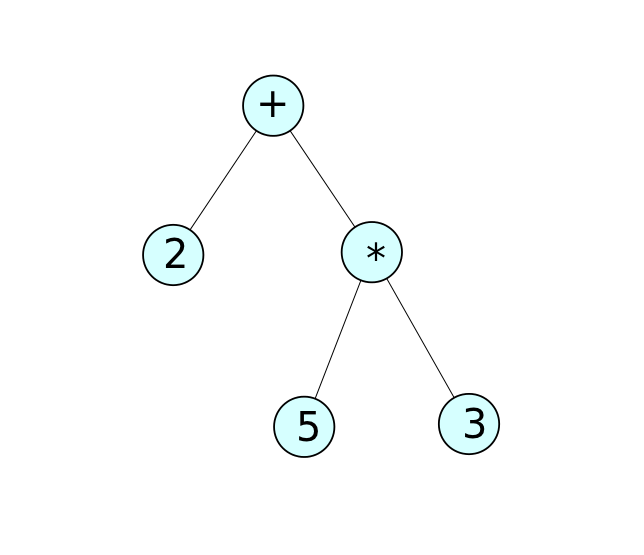
\includegraphics[width=6cm]{tree1.png}
    \caption{first tree, build from string '2+g*3'}
  \end{subfigure}
  \begin{subfigure}[b]{0.5\textwidth}
    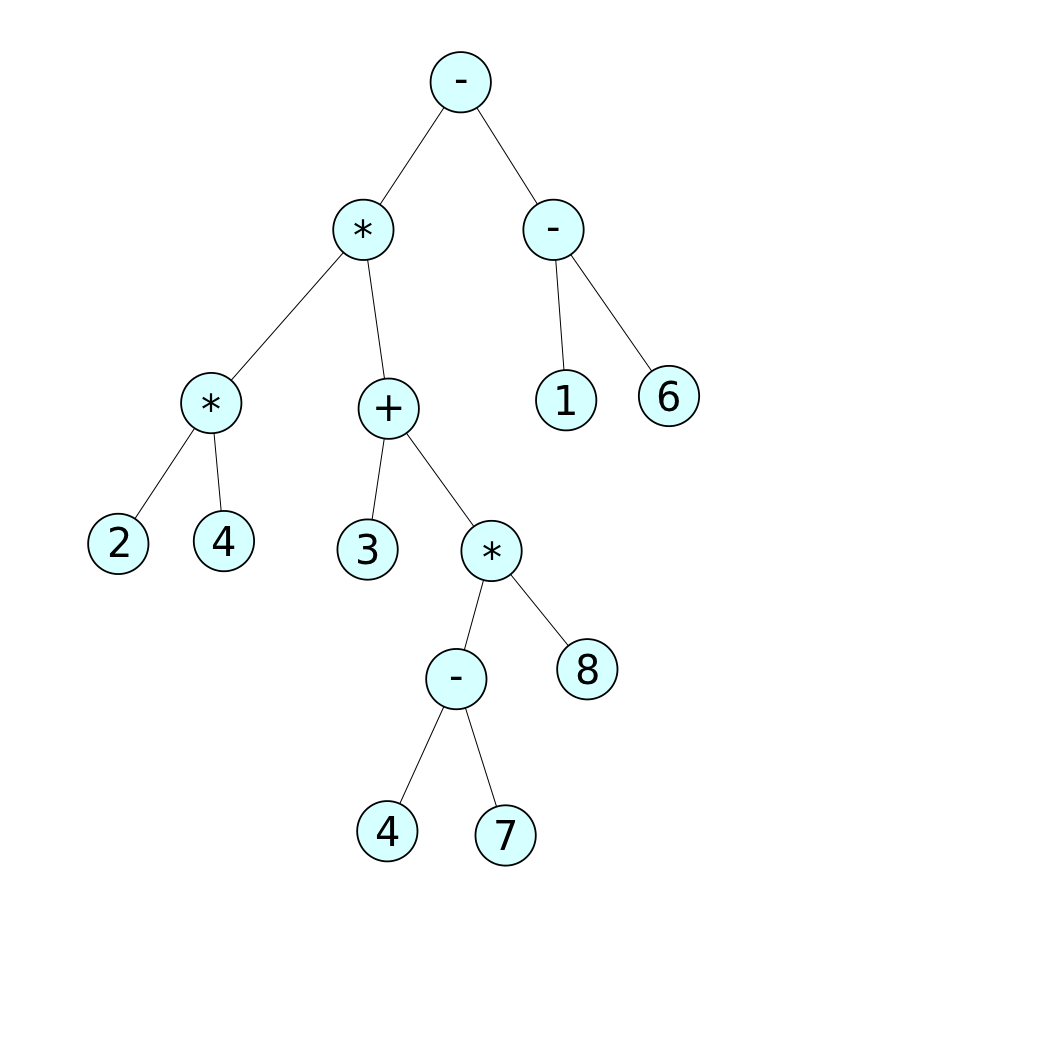
\includegraphics[width=6cm]{tree2.png}
    \caption{second tree, build from string '2*4*(3+(4-7)*8)-(1-6)'}
  \end{subfigure}
  \caption{Trees build from string expressions by algorithm described in 2a}
  \label{fig:trees}
\end{figure}


\subsection*{(2c)}


\begin{minted}{python}
dic = {'+': operator.add, '-': operator.sub, "*": operator.mul, 
       "/": operator.div, "0":0, "1":1, "2":2, "3":3, "4":4, "5":5, "6":6,
       "7":7, "8":8, "9":9}


def calculateFromTree(tree):
    """ calculate expression from tree
    """
    if tree.left.left != None: # left child is operator
        calculateFromTree(tree.left)
    if tree.right.left != None: #right child is operator
        calculateFromTree(tree.right)

    #both children are numbers -> do operation
    if tree.left.left == None and tree.right.left == None:                    
        tree.key = dic[tree.key](int(tree.left.key), int(tree.right.key))
        tree.left = None
        tree.right = None
    return tree.key


def evalString(string):
    """ evaluate expression given as string
    build tree from string, then calculate expression from tree
    no checking that input string is correct...
    """
    tree = buildTree(string)
    result = calculateFromTree(tree)

    return result
\end{minted}


%\inputminted{python}{1.2.py}



\end{document}
